\subsection{Non-linear sloshing in a rectangular container}\label{sec:Ansari}

Free surface oscillations of a liquid confined in a closed container (sloshing phenomenon) are an important issue when large amounts of liquid are industrially transported. The phenomenon involves two fluids that share a free surface boundary separating them, normally the density of the upper fluid is several orders of magnitude less than the bottom one. This phenomenon has proven of great interest due to the fact that violent impacts of the fluid can affect the structural integrity of the container.

For the studied cases in this section, the sloshing phenomenon is produced by a horizontal harmonic excitation $x = a_h \sin (\omega_h t)$, where $a_h$ is the excitation amplitude and $\omega_h$ is the excitation frequency of the rectangular tank where the two fluid phases are contained. The tank is divided in two parts, the bottom part where there is water with a density of $\rho_{I} = 1000 [kg/m^3]$ and the top part which contains a fluid with different densities $\rho_{II} = 1.3, 50, 200, 800 [kg/m^3]$, depending on the studied case. The dimensions of the tank are $a$(width) by $b$(height) and the initial free surface is at height $h$ from the bottom of the tank, see Figure \ref{fg:ansari-config}. The free surface starts the simulation as a horizontal line and is subsequently deformed by the tank excitation and the flow dynamics.

\begin{figure}[H]
  \begin{center}
      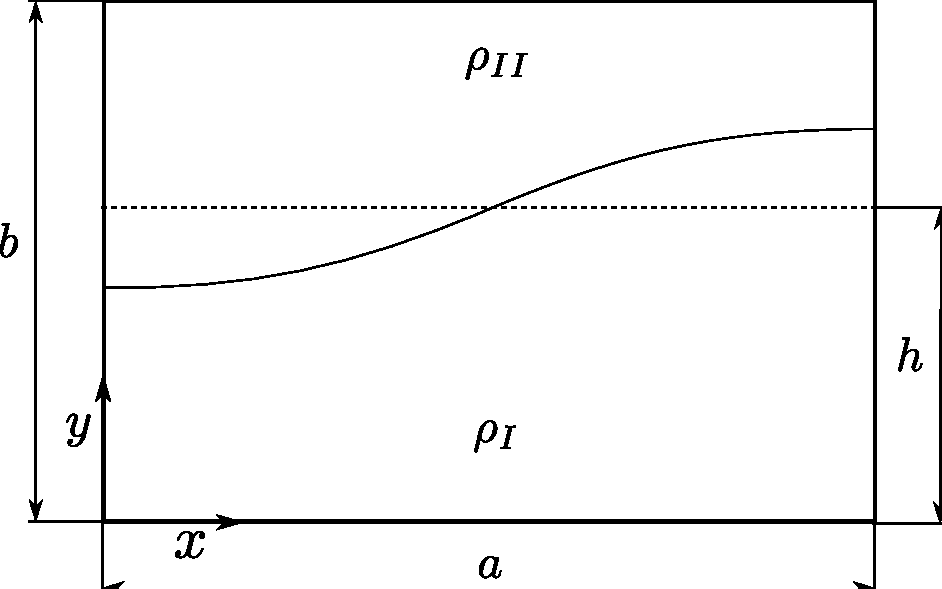
\includegraphics[width=.6\columnwidth]{images/ansari_config.pdf}
  \end{center}
  \caption{\label{fg:ansari-config} Configuration of the Non-linear sloshing in a rectangular container case. Initial condition is represented by a dashed line. The continuous line represents the position of the free-surface at a certain time.}
\end{figure}


For the different cases in this report, a 2D rectangular tank $a=1.0[m]$ width by $b=1.0[m]$ height is used. The initial height of the interface is $h=0.5[m]$ and the lateral excitation applied is $x=0.05\sin(3t)$. The simulations were performed considering the flow as laminar and non-viscous, hence, no turbulence model was included and slip boundary conditions were used. The density ratio $\sigma=\frac{\rho{II}}{\rho{I}}$ was modified to study its influence on the free surface evolution. A two dimensional Cartesian mesh of $450\times225$, splitted into triangles, has been used in all cases.

Reference results for this case are taken from \cite{Goni13} which uses the codes STARCCM+ and \OF to obtain numerical solutions and reports the free surface displacement on the left wall of the container. Those simulations use the same grid as presented above, but, in order to avoid numerical instabilities, the $CFL$ number was limited to $CFL_{max}=0.5$ which implies $\Delta t \approx 0.001$. In PFEM-2 such restrictions do not exist, $\Delta t$ is therefore fixed to $0.01$, reaching a $CFL_{max}\approx5$.
Figure \ref{fg:ansari-results} presents the free surface displacement reported on the left wall of the container for different values of $\sigma$. For each one of them, PFEM-2 simulations show a good agreement with reference solutions. It is worth mentioning that the time step used is around ten times bigger than the one used in \cite{Goni13}.


  \begin{figure}[h]
  \centering
    \subfloat[]{
	  \label{fg:ansari-1}         %% Etiqueta para la primera subfigura
	  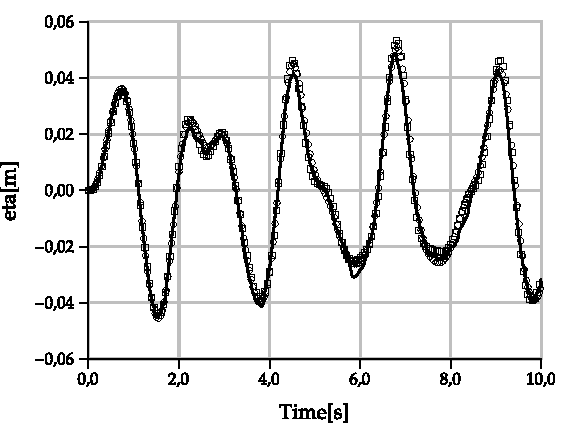
\includegraphics[width=.47\columnwidth]{images/ansari_1.pdf}
    }
    %%----segunda subfigura----
    \subfloat[]{
	  \label{fg:ansari-2}         %% Etiqueta para la segunda subfigura
	  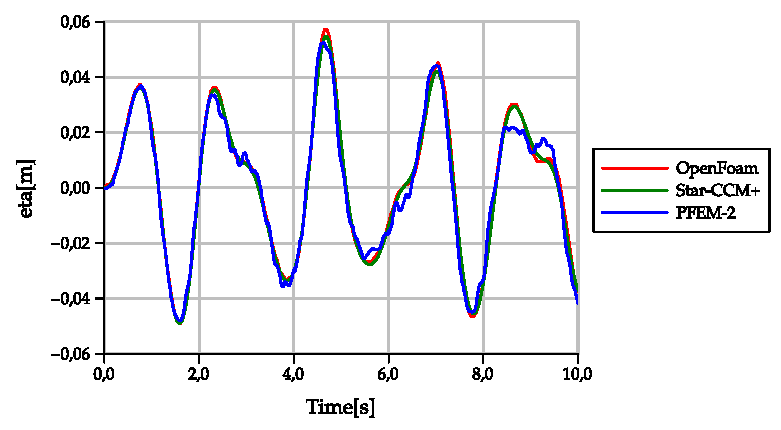
\includegraphics[width=.47\columnwidth]{images/ansari_2.pdf}
    } \\
    \subfloat[]{
	  \label{fg:ansari-3}         %% Etiqueta para la primera subfigura
	  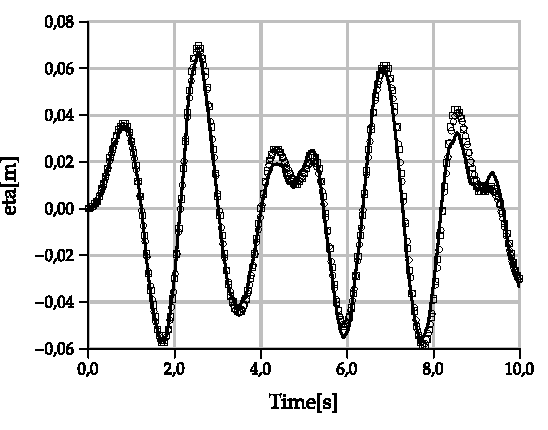
\includegraphics[width=.47\columnwidth]{images/ansari_3.pdf}
    }
    %%----segunda subfigura----
    \subfloat[]{
	  \label{fg:ansari-4}         %% Etiqueta para la segunda subfigura
	  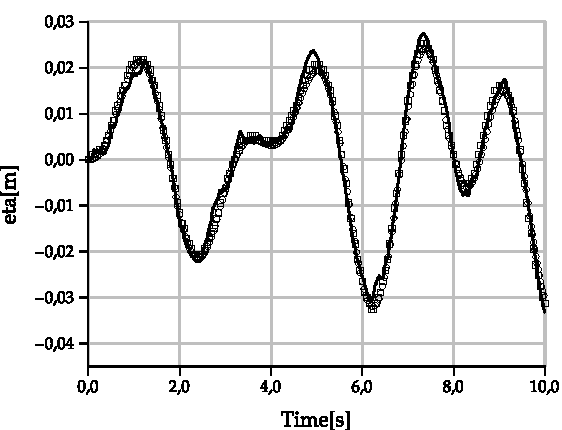
\includegraphics[width=.47\columnwidth]{images/ansari_4.pdf}
    }
   \caption{Level height on the left wall for a two phase flow for different density ratios. Figure \ref{fg:ansari-1}: $\sigma=0.0013$, Figure \ref{fg:ansari-2}: $\sigma=0.05$, Figure \ref{fg:ansari-3}: $\sigma=0.2$ and Figure \ref{fg:ansari-4}: $\sigma=0.8$. References:\ \Circle \ STARCCM, \Square \ OpenFOAM and filled line PFEM-2.}
   \label{fg:ansari-results}                %% Etiqueta para la figura entera
\end{figure}

\subsubsection{Enrichment and density ratio issues}

The PFEM-2 results presented in the previous section, have been obtained using the continuous enrichment strategy, which allows for the same formulation to be used, independently of the Froude number. However, as was mentioned before, without using a continuous formulation between elements for the enriched shape functions, the assumption about the inter-elemental boundary terms of the Poisson equation formulation should be revisited. In this subsection, problems that appear when the formulation combines non continuous enriched shape functions and large density ratio ($\rho_I/(\rho_I-\rho_{II})\sim 1$) are presented. The latter is somewhat quantified by the Froude number, which also includes the ratio between inertial and gravitational forces, this is $Fr = \dfrac{U^2}{gL}\dfrac{\rho_I}{\rho_I-\rho_{II}}$. This phenomenon is mentioned, but not investigated, by Coppola\cite{Coppola05}.

Figure \ref{fg:ansari-results-b} shows a comparison between the level height calculated by PFEM-2 using continuous enrichment, discontinuous enrichment and no-enrichment for two extreme density ratio cases. It must be noted that next results were obtained with the enrichment shape functions presented in \ref{eq:enrich-1a}, however, using \ref{eq:enrich-2a}, and condensing the elemental matrices, similar conclusions were reached. The reference solution used in Figure \ref{fg:ansari-results-b} was obtained using the formulation presented in \ref{eq:enrich-2a} without condensing, which is equivalent to continuous enrichment. As was mentioned, that reference solution was previously validated in section \ref{sec:Ansari}.

%Da la impresión que ambos sistemas de enrichment deberían ser discontinuos(??), pero el segundo es contínuo. -> Si bien el segundo sistema parece ser continuo, la continuidad va a depender de como lo ensamblas. Si haces condensación, aun utilizando el segundo enrichment te queda discontinuo. Si quieres continuidad hay que utilizar el segundo enrichment y NO condensar.

When both fluids have similar densities $\sigma \sim 1$, larger $Fr$ values are obtained. In Figure \ref{fg:ansari-4b}, a comparison with $\sigma=0.8$ between different PFEM-2 formulations is presented. When no enrichment strategy is used, the solution presents a noisy behavior where, according to the level heights, a typical mass-loss appears, deteriorating the overall solution. When discontinuous enrichment is added (this is, condensing the equation system (\ref{eqsys-poisson})) the solution is smoother but still excessively dissipative compared to the continuous enrichment formulation used as reference. Meaning that, when the discontinuous enrichment formulation is used, the assumption of avoiding the inter-elemental boundary terms in the right hand side of (\ref{poisson}) is not correct and, consequently, a diffusive behavior appears. This conclusion is confirmed when discontinuous enrichment is used (but without weakening the divergence of the velocity) and a solution very similar to the continuous enrichment one is obtained (not presented in the figure due to being almost identical to the reference). By not integrating by parts, the divergence term requires imposing a pressure gradient on the boundaries: if large density ratios are used, the previous gradient value $\nabla p^n$ can be imposed on the boundaries, although this approximation is not valid when there is a gravitational field, low density ratio and the fluid is not at rest.


For the other limit $\sigma \ll 1$, the case when $\sigma=0.0013$, is presented in Figure \ref{fg:ansari-1b}. The graphic shows that both the continuous and the discontinuous enrichment solutions present a very similar behavior. As before, when no enrichment is used, results become noisy, showing that a spurious velocity field appears close to the free surface when no improvements are introduced in this region. Discontinuous enrichment with a strong form of divergence of the velocity cannot be used in this case due to the wrong prediction of the pressure gradients on the boundaries which turns the simulation unstable.

  \begin{figure}[h]
  \centering
    \subfloat[]{
	  \label{fg:ansari-1b}         %% Etiqueta para la primera subfigura
	  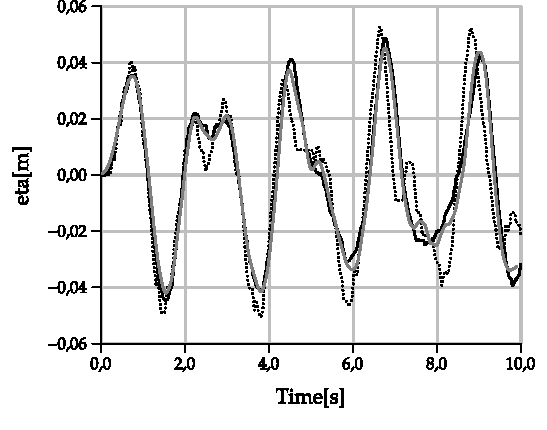
\includegraphics[width=.49\columnwidth]{images/ansari_1b.pdf}
    }
    %%----segunda subfigura----
    \subfloat[]{
	  \label{fg:ansari-4b}         %% Etiqueta para la segunda subfigura
	  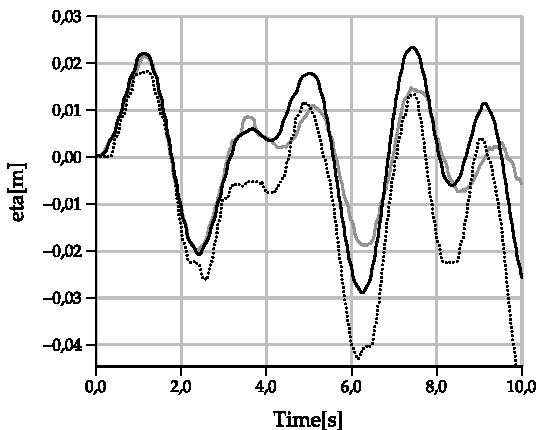
\includegraphics[width=.49\columnwidth]{images/ansari_4b.pdf}
    }
   \caption{Level height on the left wall of a two phase flow for different density ratios. Figure \ref{fg:ansari-1b}: $\sigma=0.0013$ and Figure \ref{fg:ansari-4b}: $\sigma=0.8$. References: filled black line continuous enrichment, filled gray line discontinuous enrichment, and dotted line without enrichment.}
   \label{fg:ansari-results-b}                %% Etiqueta para la figura entera
\end{figure}

In the current implementation, choosing the continuous enrichment formulation increases the total CPU time by $50\%$ compared to the other discontinuous formulations, albeit with the great advantage of being applicable to a wide range of situations. If the discontinuous enrichment formulation is used, better computing times are obtained. Nonetheless, some particularities, such as integrating the velocity divergence term by parts or not, must be taken into account depending on the density ratio of the problem.

\clearpage
